\gls{tic} is a tool totally devoted to the \gls{tc} RNA-Seq data offering features to inspect data, to normalize them, to capture differential expression of genes at static time point and overall time points, supporting different experimental designs.

Moreover, it's possible to compare the results of different analysis and to investigate the most influenced biological functions (i.e. Gene Ontology terms and Pathways). 

Overall, \gls{tic} offers gives the possibility to analyze data using different R packages, to compare the results in order to choose the best combination of tools for the user specific problem. Therefore, \gls{tic} offers a vast amount of exploratory and diagnostic interactive plots to explore data not just at pre-processing but also during the post-processing phase. 

\gls{tic} automatically implements a set of Reproducible Research functionalities to trace all the analysis steps selected by the user, generating a final report with both executed analysis code chunks and their produced results. Furthermore, \gls{tic} has been provided also of a caching system providing, for each analysis step, a caching database file within all the input and output processed data, useful, not only to speed up computations, but also to share data and results through the Internet.




gives the possibility to analyse time course RNA-Seq data starting from \textit{BAM} files.
It enables RNA expression quantification with \lstinline!featureCounts! method producing a count matrix useful for \glspl{deg} detection.

We gave particular attention to the normalization phase, giving the possibliity not only to use several traditional normalizations methods, but also the possiblity to remove batch effect.


\begin{figure}[H]
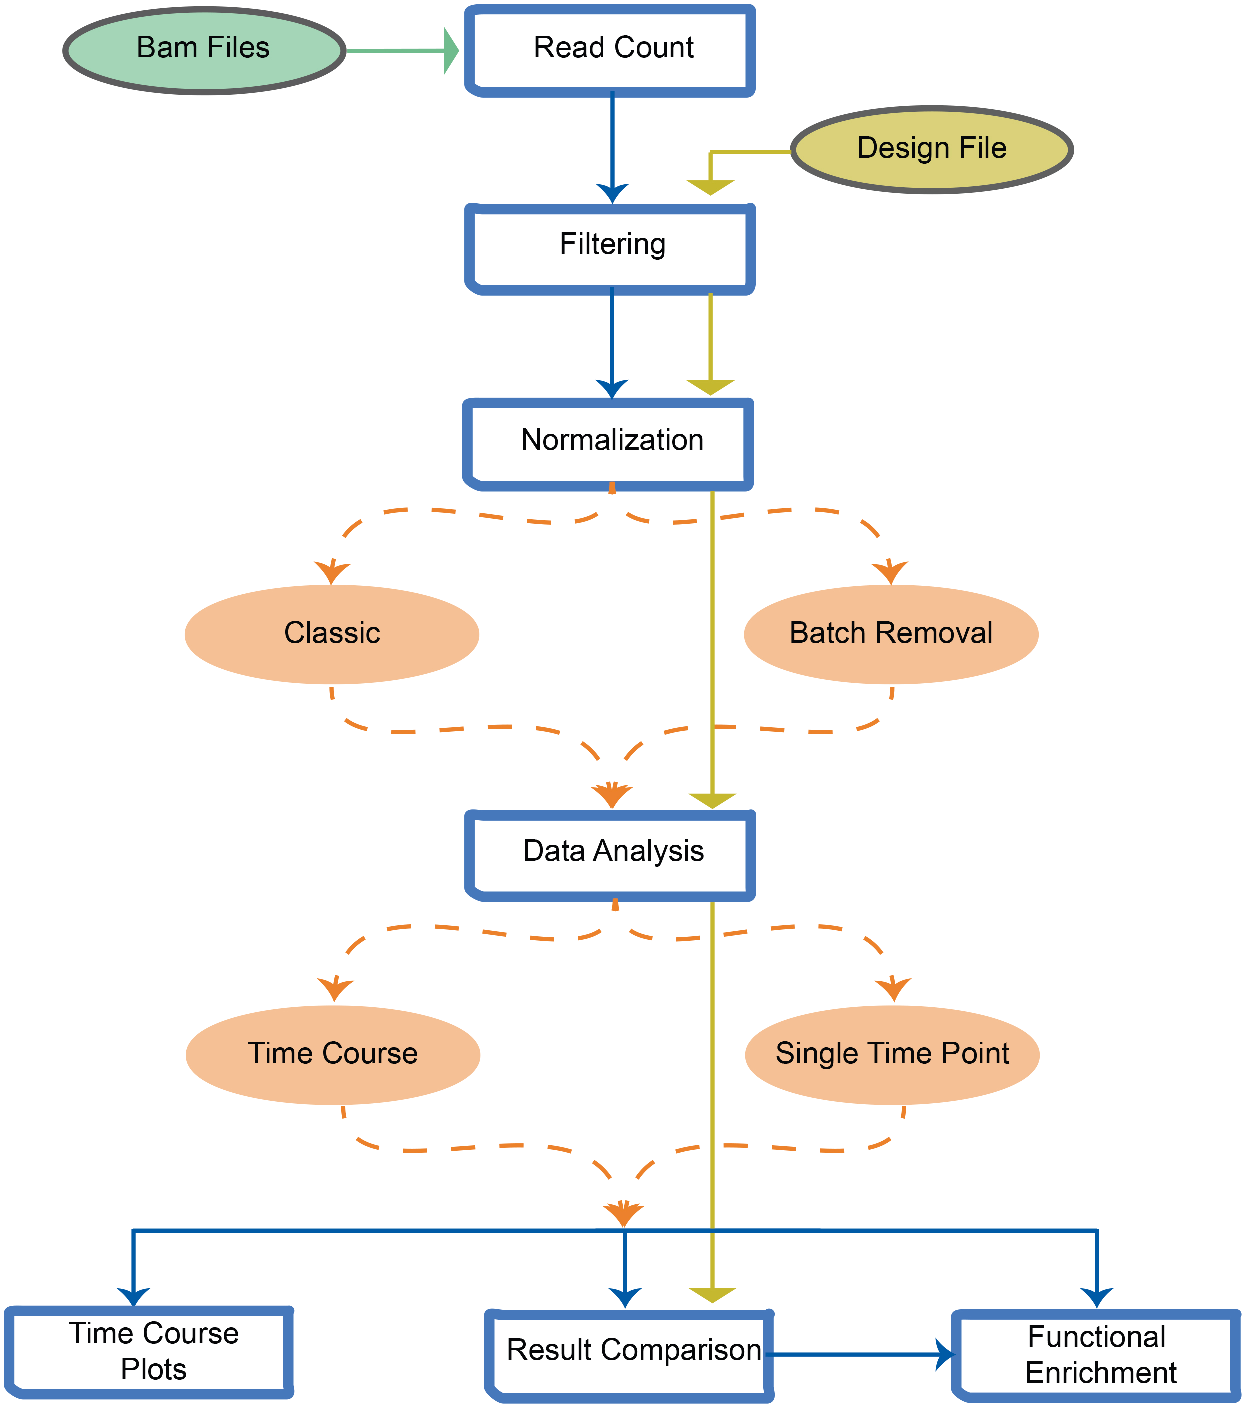
\includegraphics[width=\textwidth,height=\textheight,keepaspectratio]{img/ticorser/main_flow.pdf}
\caption[ticorser mainflow]{Main flow of ticorser R package.}
\label{fig:ticorserflow}
\centering
\end{figure}

\gls{tic} offers four different ways for analyzing time course RNA-Seq data.

Moreover, it offers three different ways for analyzing different biological conditions in a single time point.